%%%%%%%%%%%%%%%%%%%%%%%%%%%%%%%%%%%%%%%%%
% Focus Beamer Presentation
% LaTeX Template
% Version 1.0 (8/8/18)
%
% This template has been downloaded from:
% http://www.LaTeXTemplates.com
%
% Original author:
% Pasquale Africa (https://github.com/elauksap/focus-beamertheme) with modifications by
% Vel (vel@LaTeXTemplates.com)
%
% Template license:
% GNU GPL v3.0 License
%
% Important note:
% The bibliography/references need to be compiled with bibtex.
%
%%%%%%%%%%%%%%%%%%%%%%%%%%%%%%%%%%%%%%%%%

%----------------------------------------------------------------------------------------
%	PACKAGES AND OTHER DOCUMENT CONFIGURATIONS
%----------------------------------------------------------------------------------------

\documentclass{beamer}
\usepackage[ngerman]{babel}
\usepackage{xcolor}

\definecolor{hmred}{RGB}{251, 86, 85}
\usepackage{leftidx}
\usepackage{filecontents}
\usepackage{graphicx}
\usepackage{tikz}
\usepackage{pgfplots}
\usepackage{amsthm}
\usepackage{amsmath}
\usepackage{amssymb}
\usepgfplotslibrary{groupplots}



\usetheme{focus} % Use the Focus theme supplied with the template
% Add option [numbering=none] to disable the footer progress bar
% Add option [numbering=fullbar] to show the footer progress bar as always full with a slide count

% Uncomment to enable the ice-blue theme
%\definecolor{main}{RGB}{92, 138, 168}
%\definecolor{background}{RGB}{240, 247, 255}

%------------------------------------------------

\usepackage{booktabs} % Required for better table rules

% [noframenumbering] frame without number
% [plain] frame without header
%----------------------------------------------------------------------------------------
%	 TITLE SLIDE
%----------------------------------------------------------------------------------------

\title{CART-Klassifikator}

\subtitle{Pattern Matching \& Machine Learning}

\author{F. Freter, E. Kirchberger,\\S. Symhoven \& J. Wustl}

\institute{Sommersemester 2023}

\titlegraphic{
\includegraphics[scale=0.305]{Images/hmlogo.png} \\ \textcolor{hmred}{Hochschule München \\ University of Applied Sciences \\ Fakultät für
Informatik und Mathematik}} % Optional title page image, comment this line to remove itt

\date{20. Juni 2022}


%------------------------------------------------

\begin{document}



%------------------------------------------------

\begin{frame}
	\maketitle % Automatically created using the information in the commands above
\end{frame}

%------------------------------------------------

\begin{frame}{Inhalt}
	\tableofcontents % Automatically created using the information in the commands above
\end{frame}


%----------------------------------------------------------------------------------------
%	 SECTION 1
%----------------------------------------------------------------------------------------


\section{Training und Aufbau des Baumes}
 
\begin{frame}{CART: Classification And Regression Trees}
	\begin{itemize}
		\item {\textbf{Decision Trees}: Graphische Darstellung von Entscheidungen}
		\item{\textbf{Zweck}: Vorhersage von kategorischen oder kontinuierlichen Zielvariablen}
		\item{\textbf{Trainingsdaten}: Beispiele mit Merkmalen und Zielvariablen}
		\item{\textbf{Überwachtes Lernverfahren}: Anwendungen von medizinischer Diagnostik bis Kreditrisikobewertung}
		\item{\textbf{Verzweigungsknoten}: Auswahl zwischen Alternativen}
		\item{\textbf{Blattknoten}: Finale Entscheidung (Vorhersage)}
		\item{\textbf{CART-Algorithmen}: \textbf{Klassifizierung} (kategorisch) und \textbf{Regression} (kontinuierlich)}
	\end{itemize}		
	
	\pause
	\begin{alertblock}{Classification Trees}
		Im Folgenden fokussieren wir uns auf die  \textbf{Classification Trees}.
	\end{alertblock}
\end{frame}

\begin{frame}{Aufbau eines Classification Trees}

	\begin{columns}
		\column{0.5\textwidth}
			\begin{itemize}
				\item {\textbf{Root Node}: Startpunkt, enthält alle Daten und startet die Unterteilung (basierend auf Merkmal mit Informationsgewinn).}
				\item {\textbf{Decision Node}: Teilt Daten weiter auf, basierend auf Merkmalen.}
				\item {\textbf{Leaf Node}: Endpunkte repräsentieren finale Vorhersagen (basierend auf Merkmalen des gegebenen Datenpunkts). Keine weiteren sinnvollen Teilungen möglich.}
			\end{itemize}	
			
		\column{0.5\textwidth}
			\begin{figure}
				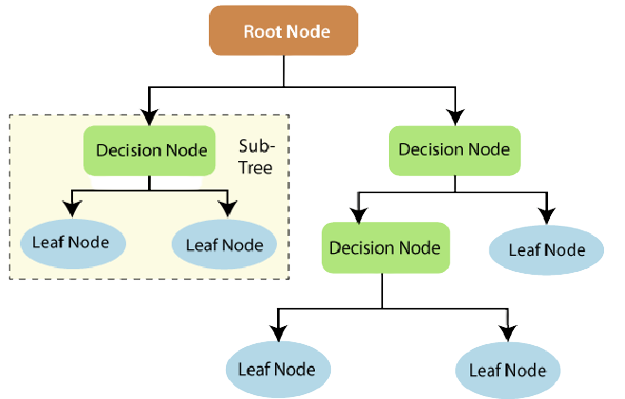
\includegraphics[width=\linewidth]{Images/tree.png}
				\caption{Decision Tree \cite{Charbuty2021ClassificationBO}}
			\end{figure}
			
			\pause
			\begin{alertblock}{Ziel}
				Optimale Vorhersagen auf Basis von Eingangsmerkmalen.			
			\end{alertblock}
	\end{columns}

\end{frame}

\begin{frame}{Strategie}
	\begin{itemize}
		\item{\textbf{Allgemeine Strategie}: Eingangsdaten werden in $P$ disjunkte Regionen $R_1,\dots,R_P$ aufgeteilt.}
		\item{Jede Region stellt eine Entscheidungsklasse dar.}
		\item{Für jede Region wird die am häufigsten vorkommende Klasse als Vorhersage gewählt.}
		\item{Bewertungsmaße wie Gini-Index oder Entropie bestimmen den besten Split.}
	\end{itemize}
	
	\begin{columns}
		\column{0.5\textwidth}
			\begin{itemize}
				\item{\textbf{Rekursiver Algorithmus}:}
				\begin{itemize}
					\item {Aufteilung des Ausgangsraums $R$ in $R_1$ und $R_2$}
					\item{Suche nach der besten Aufteilung für $R_1$ und $R_2$}
					\item{Wiederhole für alle erzeugten Regionen}
				\end{itemize}
			\end{itemize}
			
		\column{0.43\textwidth}
			\begin{figure}
				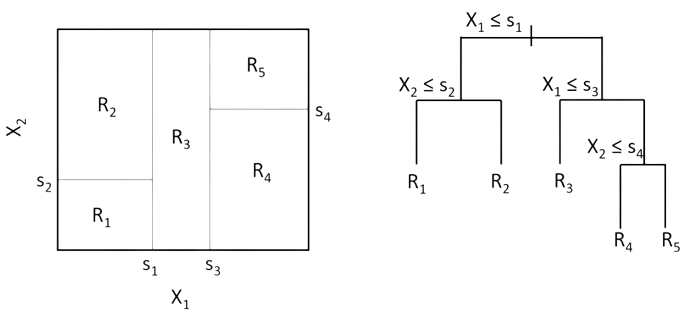
\includegraphics[width=\linewidth]{Images/split.png}
				\caption{Rekursive Teilung \cite{hastie_tibshirani_friedman}}
			\end{figure}
	\end{columns}
	
\end{frame}

\begin{frame}{Vorgehen bei einem Klassifikationsproblem}
	\begin{itemize}
		\item {Ziel: Vorhersage der Klassenlabel.}
		\item {Jeder Knoten repräsentiert eine Entscheidung basierend auf einer Variable.}
		\item {Für jede Aufteilungsvariable werden alle möglichen Aufteilungspunkte betrachtet.}
		\item {Bewertungsmaße wie Gini-Index oder Informationsgewinn bestimmen die beste Aufteilung.}
		\item {Die Aufteilungsvariable und der Aufteilungspunkt, die das optimale Bewertungsmaß erzielen, werden ausgewählt.}
		\item {Dieser Prozess wird rekursiv fortgesetzt, bis eine bestimmte Stopp-Regel erfüllt ist (z.B. maximale Tiefe, minimale Anzahl von Instanzen pro Blatt, usw.).}
		\item {Jeder Blattknoten repräsentiert eine Klasse; eine neue Beobachtung wird entsprechend klassifiziert.}
	\end{itemize}
\end{frame}

%----------------------------------------------------------------------------------------
%	 SECTION 2
%----------------------------------------------------------------------------------------

\section{Bewertungsmaße für einen Split}
%------------------------------------------------

\begin{frame}{Bewertungsmaße: Gini-Index, Informationsgewinn \& Missclassification Error}
	\begin{itemize}
		\item{\textbf{Gini-Index}}
		\begin{itemize}
			\item Maß der Unreinheit einer Gruppe
			\item $Gini = 1 - \sum_{i=1}^k p_i^2$, wobei $p_i$ die Wkt. der Klasse $i$ ist.
			\item \textbf{Ziel}: Minimierung des gewichteten Gini-Indexes.
		\end{itemize}
		\item{\textbf{Informationsgewinn}}
		\begin{itemize}
			\item Reduktion der Entropie durch den Split
			\item $IG = H(parent) - \sum_{j=1}^m \frac{n_j}{n} H(child_j)$, wobei $H$ die Entropie ist.
			\item \textbf{Ziel}: Maximierung des Informationsgewinns.
		\end{itemize}
		\item{\textbf{Missclassification Error}}
		\begin{itemize}
			\item {Der Misclassification Error (ME) ist ein Maß für die Fehlklassifizierung.}
			\item {$ME = 1 - \max(p_1, p_2, \dots, p_k)$, wobei $p_i$ die Wkt. der Klasse $i$ ist.}
			\item {ME kann als Bewertungsmaß für die Baumkonstruktion verwendet werden.}
			\item {\textbf{Ziel}: Minimierung des gewichteten Missclassification Errors.}
		\end{itemize}
	\end{itemize}
\end{frame}

%----------------------------------------------------------------------------------------
%	 SECTION 3
%----------------------------------------------------------------------------------------

\section{Auswertung des Modells}

\begin{frame}{Auswertung des Modells}
	\begin{itemize}
		\item {Unvoreingenommene Schätzung der Modellleistung durch Kreuzvalidierung oder separate Testdatensätze.}
		\item {Gebräuchliche Metriken für binäre Klassifikation: Genauigkeit, Präzision, Recall, F1-Score und AUC-ROC.}
		\item {Genauigkeit: Verhältnis der korrekten Vorhersagen zu den gesamten Vorhersagen.}
		\item {Präzision: Verhältnis der wahren Positiven zu der Summe aus wahren und falschen Positiven.}
		\item {Recall: Verhältnis der wahren Positiven zu der Summe aus wahren Positiven und falschen Negativen.}
		\item {F1-Score: harmonisches Mittel von Präzision und Recall.}
		\item {AUC-ROC: Zusammenfassung der Klassifikationsleistung über alle möglichen Klassifikationsschwellen.}
		\item {Overfitting-Vermeidung durch Techniken wie Pruning oder Regularisierung.}
	\end{itemize}
\end{frame}

%----------------------------------------------------------------------------------------
%	 SECTION 4
%----------------------------------------------------------------------------------------

\section{Overfitting und Pruning}

\begin{frame}{Overfitting in Decision Trees}
	\begin{itemize}
		\item {Ein vollständig gewachsener Decision Tree kann überangepasst sein (\textbf{Overfitting}).}
		\item {Dies kann durch Rauschen oder einen Mangel an repräsentativen Daten verursacht werden.}
		\item {\textbf{Ziel}: Erstellung eines Modells, das gut auf neue, ungesehene Daten verallgemeinert.}
	\end{itemize}
\end{frame}

\begin{frame}{Vermeidung von Overfitting}
	\begin{itemize}
		\item {Das Wachstum des Baums kann vorzeitig gestoppt werden.}
		\item {Alternativ kann der Baum zunächst vollständig wachsen und anschließend beschnitten werden (\textbf{Pruning}).}
		\item {Verschiedene Pruning-Methoden: Reduced Error Pruning, Minimum Description Length Pruning, Cost-Complexity Pruning.}
	\end{itemize}
\end{frame}

\begin{frame}{Cost-Complexity Pruning}
	\begin{itemize}
		\item {\textbf{Ziel}: Verhindern von Overfitting durch Entfernen von Zweigen, die wenig zur Vorhersageleistung beitragen}
		\item {\textbf{Kostenkomplexitätspruning}: Gleichgewicht zwischen Baumgröße und Trainingsfehler}
		\item \textbf{Kostenkomplexitätskriterium}: \[C_{\alpha}(T) = C(T) + \alpha|T|, \, mit\]
		\begin{itemize}
			\item $C(T)$ ist der Misclassification Error des Baumes $T$.
			\item $|T|$ ist die Anzahl der terminalen Knoten des Baumes $T$.
			\item $\alpha$ ist ein Komplexitätsparameter, der die Präferenz zwischen Baumgröße und Trainingsfehler steuert.
		\end{itemize}
		\item Durch Variieren von $\alpha$ kann eine Sequenz optimaler Bäume ermittelt werden.
		\item Kreuzvalidierung kann verwendet werden, um den optimalen Wert von $\alpha$ zu bestimmen.
	\end{itemize}
\end{frame}


%----------------------------------------------------------------------------------------
%	 SECTION 5
%----------------------------------------------------------------------------------------

\section{Vor- und Nachteile}

\begin{frame}
	\begin{columns}[T, onlytextwidth]
		\column{0.5\textwidth}
			\textbf{Vorteile}:
			\begin{itemize}
				\item leicht zu trainieren
				\item leicht zu interpretieren
				\item einfach zu visualisieren
				\item können mit verschiedenen Prädiktoren umgehen \\$\rightarrow$ keine Dummies erforderlich
			\end{itemize}
		
		\column{0.5\textwidth}
			\textbf{Nachteile}:
			\begin{itemize}
				\item nicht die besten Lerner
				\item reagieren empfindlich auf sich ändernde Trainingsdaten
				\item werden von den oben genannten Splits dominiert \\$\rightarrow$ erster Split beeinflusst stark die Form des gesamten Baums
			\end{itemize}
	\end{columns}
\end{frame}

%----------------------------------------------------------------------------------------
%	 SECTION 6
%----------------------------------------------------------------------------------------

\section{Verbesserungsmöglichkeiten \& Ausblick}

\begin{frame}
		\begin{itemize}
			\item\textbf{Stacking}: Ensemble-Lern-Technik. Mehrere CART-Modelle kombiniert werden. Ausgaben der einzelnen Modelle  werden als Eingabe für ein Meta-Modell verwendet.
			\item\textbf{Bayesian Model Averaging}: Modellselektion. Mehrere Modelle auf der Grundlage von Bayes'schen Wahrscheinlichkeiten kombiniert werden.
			\item\textbf{Bagging}: Ensemble-Lern-Technik. Mehrere CART-Modelle werden auf unterschiedlichen Stichproben der Daten trainiert.
			\item\textbf{Random Forests}: Ensemble-Lern-Modell. Besteht aus vielen unkorrelierten Entscheidungsbäumen, die auf zufälligen Untergruppen der Daten trainiert werden.
			\item\textbf{Boosting}: Ensemble-Lern-Technik. Sequentielle Anordnung von schwachen CART-Modellen, wobei jeder Baum versucht, die Fehler des vorherigen Baums zu korrigieren.
		\end{itemize}
\end{frame}


%----------------------------------------------------------------------------------------
%	 CLOSING/SUPPLEMENTARY SLIDES
%----------------------------------------------------------------------------------------

\appendix

\begin{frame}[allowframebreaks]{References}
	\bibliography{references.bib}
	\nocite{*}
	\bibliographystyle{plain}
\end{frame}

\begin{frame}[focus]

	Fragen, Kritik oder Anregungen?
	
\end{frame}

%----------------------------------------------------------------------------------------

\end{document}
